\documentclass[a4paper, 12pt]{article}

% english
\usepackage[english]{babel}
\usepackage{lmodern}


% biblio
%\usepackage{csquotes}
%\usepackage[backend=biber, language=english]{biblatex}
%\addbibresource{./biblio.bib}

% packages
\usepackage{fullpage}				% really narrow margins
\usepackage{graphicx}				% \includegraphics
\usepackage{amsmath}				% \text
\usepackage{multirow}				% \multirow		
\usepackage{enumitem}				% \setitemsize
\usepackage{appendix}				% appendix env
\usepackage{pgf, tikz}			% figures
\usepackage{hhline}

% center vertically
\usepackage{titling}				
\renewcommand\maketitlehooka{\null\mbox{}\vfill}
\renewcommand\maketitlehookd{\vfill\null}

% figures
\usetikzlibrary{positioning}

% misc
\addto\captionsenglish{\def\chaptername{Part}}		% Part/Chapter
\renewcommand\thesection{\arabic{section}}				% arabic numbers
\setlength\parindent{0pt}													% no indentation
\setitemize{itemsep=0em}													% no space between itms

% code (default C++)
\usepackage{listings}
\usepackage{xcolor}
\definecolor{keyword}{rgb}{0.76,0.18,0.64}
\definecolor{directive}{rgb}{0.47,0.28,0.18}
\definecolor{string}{rgb}{0.85,0.16,0.14}
\definecolor{comment}{rgb}{0.43,0.65,0.38}
\lstdefinestyle{cpp}{
  language=C++,
  tabsize=2,
  keepspaces=true,
  showspaces=false,
  showtabs=false,
  showstringspaces=false,
  basicstyle=\ttfamily\footnotesize,
  keywordstyle=\color{keyword}\ttfamily,
  stringstyle=\color{string}\ttfamily,
  commentstyle=\color{comment}\ttfamily,
  morecomment=[l][\color{directive}]{\#}
}
%\lstdefinestyle{xml}{
%  language=C++,
%  tabsize=2,
%  keepspaces=true,
%  showspaces=false,
%  showtabs=false,
%  showstringspaces=false,
%  basicstyle=\ttfamily\footnotesize,
%  stringstyle=\color{string},
%  identifierstyle=\color{directive},
%  keywordstyle=\color{directive},
%  morestring=[b]",
%  moredelim=[s]{>}{<},
%  morecomment=[s]{<?}{?>},
%  morekeywords={} % list attr here
%}


\title{C++}
\date{}

\begin{document}

\maketitle
\tableofcontents

\section{Inheritance}

	\subsection*{\texttt{public}, \texttt{protected} and \texttt{private} inheritance}

We can summarize the different access types according to which functions can access them in the following way:
\begin{center}
\begin{tabular}{| p{7cm} | c | c | c |}
\cline{2-4}
\multicolumn{1}{c |}{} & \texttt{public} & \texttt{protected} & \texttt{private} \\
\hline
members of the same class & X & X & X \\
\hline
members of derived class & X & X & \\
\hline
not members & X & & \\
\hline
\end{tabular}
\end{center}

The same happens with \texttt{public}, \texttt{private} and \texttt{protected} inheritance. Let's consider a class \texttt{Base} and a class \texttt{Child} that inherits from \texttt{Base}. We can summarize who is aware of the inheritance in the following way:

\begin{center}
\begin{tabular}{| p{7cm} | c | c | c |}
\cline{2-4}
\multicolumn{1}{c |}{} & \texttt{public} & \texttt{protected} & \texttt{private} \\
\hline
\texttt{Child} & X & X & X \\
\hline
\texttt{Child}'s children & X & X & \\
\hline
everything that is aware of \texttt{Base} and \texttt{Child} & X & & \\
\hline
\end{tabular}
\end{center}

~\\\indent
In principle, a publicly derived class inherits access to every member of a base class except:
\begin{itemize}
	\item its constructors and its destructor
	\item its assignment operator members (operator=)
	\item its friends
	\item its private members
\end{itemize}

Even though access to the constructors and destructor of the base class is not inherited as such, they are automatically called by the constructors and destructor of the derived class.

Unless otherwise specified, the constructors of a derived class calls the default constructor of its base classes (i.e., the constructor taking no arguments). Calling a different constructor of a base class is possible, using the same syntax used to initialize member variables in the initialization list:

\begin{lstlisting}[style=cpp][style=cpp]
	Derived(parameters) : Base(parameters) {...}
\end{lstlisting}

	\subsection*{Overloading in Derived Classes}

In C++, there is no overloading across scopes -- derived class scopes are not an exception to this general rule:

\begin{lstlisting}[style=cpp]
	class Base {
   public:
    int f(int i) { cout << "f(int): "; return i+1; }
	};
	class Derived : public Base {
   public:
    double f(double d) { cout << "f(double): "; return d+1.3; }
 	};
	int main() {
		Derive *pd = new Derived;
		cout << pd->f(2) << endl;
		cout << pd->f(2.3) << endl;
	}
\end{lstlisting}

This produces:
\begin{verbatim}
    f(double): 3.3   // not f(int): 3
    f(double): 3.6   // as expected
\end{verbatim}

Creating an overload set of all the \texttt{f()} functions from the Base and Derived class is easily done using a using-declaration, with the keyword \texttt{using}, which asks to bring the functions into the scope:

\begin{lstlisting}[style=cpp]
	class Derived : public Base {
   public:
    using Base::f; // make every f from Base available
    double f(double d) { cout << "f(double): "; return d+1.3; }
	};
\end{lstlisting}

	\subsection*{Prevent the Inheritance From a Class}
	
It is possible by declaring the class \texttt{final}. It can be useful for efficiency, to avoid the function calls being virtual, or for safety, to ensure that the class is not used as a base class (for example, to be sure that it is possible to copy objects without fear of slicing).
	
	\subsection*{Prevent the Overriding of a Member Function}
	
Again possible by declaring the function \texttt{final}.

	\subsection*{Virtual Destructor}
	
In order to define a virtual destructor, add the keyword \texttt{virtual} before the tilde symbol of the destructor's declaration. One important design paradigm of class design is that if a class has one or more virtual functions, then that class should also have a virtual destructor.

\begin{lstlisting}[style=cpp]
	class Base {
   public:
    Base() { cout << "Constructing Base"; }
    ~Base() { cout << "Destroying Base"; }
	};
	class Derived : public Base {
   public:
    Derived() { cout << "Constructing Derived"; }
    ~Derived() { cout << "Destroying Derived"; }
 	};
	void main() {
		Base *basePtr = new Derived();
		delete basePtr;
	}
\end{lstlisting}
	
As it is now, the destructor for the \texttt{Derive} class is not being called. In order to solve it, it is possible to set the destructor for the class \texttt{Base} virtual:
\begin{lstlisting}[style=cpp]
virtual ~Base() { cout << "Destroying Base"; }

Constructing Base  
Constructing Derive
Destroying Derive     // was missing before
Destroying Base
\end{lstlisting}

	\subsection*{Virtual Constructor}
	
Doesn't exist in C++, doesn't make sense at all.
	
	\subsection*{Call to Virtual Functions in Constructors and Destructors}
	
Calling virtual functions from a constructor or destructor is dangerous and should be avoided whenever possible. All C++ implementations should call the version of the function defined at the level of the hierarchy in the current constructor and no further. Explanation with the following code:

\begin{lstlisting}[style=cpp]
	class Base {
   public:
    Base(const string& ss) { cout << "Base const\n"; f(ss); }
    virtual void f(const string&) { cout << "Base::f\n"; }
	};
	class Derived: public Base {
   public:
    Derived(const string& ss) : Base(ss) { cout << "Derive const\n"; }
    void f(const string& ss) { cout << "Derived::f\n"; s = ss; }
   private:
    string s;
	};
	int main() {
		Derived derive("Hello");
	}
\end{lstlisting}

The above program compiles and produce the following output:

\begin{verbatim}
    Base const
    Base::f
    Derive const
\end{verbatim}

Note not \texttt{Derive::f}. Consider what would happen if the rule were different so that \texttt{Derive::f()} was called from \texttt{Base::Base()}. Because the constructor \texttt{Derive::Derive()} hadn't yet been run, \texttt{Derive::f()} would try to assign its argument to an uninitialized string \texttt{s}. The result would most likely be an immediate crash. So fortunately the C++ language doesn't let this happen: it makes sure any call to \texttt{this->f()} that occurs while control is flowing through Base's constructor will end up invoking \texttt{Base::f()}, not the override \texttt{Derive::f()}.

Destruction is done "derived class before base class", so virtual functions behave as in constructors: Only the local definitions are used -- and no calls are made to overriding functions to avoid touching the (now destroyed) derived class part of the object.

  \subsection*{Order of calls to Constructors and Destructors}

Constructors are called from Base class to Derived class, and Destructors are called from Derived class to Base class.

  \subsection*{v-Table}

\begin{figure}[h]
  \center
  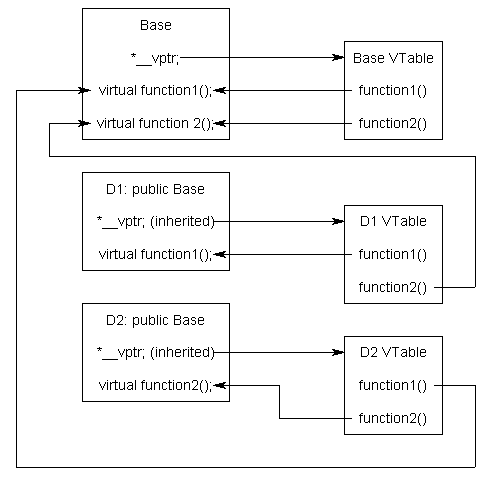
\includegraphics[width=12cm, height=10cm]{vtable.png}
  \caption{v-Table}
  \label{fig:Filevtablegif}
\end{figure}

\section{Classes}

	\subsection*{Copy Constructor}

The assignment operator is used to copy the values from one object to another already existing object. The key words here are already existing. Consider the following example:

\begin{lstlisting}[style=cpp]
	Cents cMark(5); // calls Cents constructor
	Cents cNancy; // calls Cents default constructor
	cNancy = cMark; // calls Cents assignment operator
\end{lstlisting}

In this case, cNancy has already been created by the time the assignment is executed. Consequently, the \texttt{Cents} assignment operator is called. The assignment operator must be overloaded as a member function.

What happens if the object being copied into does not already exist? To understand what happens in that case, we need to talk about the copy constructor. Consider the following example:

\begin{lstlisting}[style=cpp]
	Cents cMark(5); // calls Cents constructor
	Cents cNancy = cMark; // calls Cents copy constructor!
\end{lstlisting}
Because the second statement uses an equals symbol in it, you might expect that it calls the assignment operator. However, it doesn?t! It actually calls a special type of constructor called a copy constructor. A copy constructor is a special constructor that initializes a new object from an existing object.

The purpose of the copy constructor and the assignment operator are almost equivalent -- both copy one object to another. However, the assignment operator copies to existing objects, and the copy constructor copies to newly created objects.
	
The copy constructor should have one of the following signature:
\begin{lstlisting}[style=cpp]
	MyClass(const MyClass& other);
	MyClass(MyClass& other);
	MyClass(volatile const MyClass& other);
	MyClass(volatile MyClass& other);
  \end{lstlisting}

If you do not declare a copy constructor, the compiler gives you one implicitly. The implicit copy constructor does a member-wise copy of the source object. In many cases, this is sufficient. However, there are certain circumstances where the member-wise copy version is not good enough. By far, the most common reason the default copy constructor is not sufficient is because the object contains raw pointers and you need to take a "deep" copy of the pointer. That is, you don't want to copy the pointer itself; rather you want to copy what the pointer points to. Why do you need to take "deep" copies ? This is typically because the instance owns the pointer; that is, the instance is responsible for calling delete on the pointer at some point (probably the destructor). If two objects end up calling delete on the same non-NULL pointer, heap corruption results.

Although using the assignment operator is fairly straightforward, correctly implementing an overloaded assignment operator can be a little more tricky than you might anticipate. There are two primary reasons for this. First, there are some cases where the assignment operator isn?t called when you might expect it to be. Second, there are some issues in dealing with dynamically allocated memory (which we will cover in the next lesson).

	\subsection*{Interface}
	
An interface is a class with only pure virtual methods:
\begin{lstlisting}[style=cpp]
	class Interface {
   public:
    // Empty virtual destructor for proper cleanup
    virtual ~Interface() {}

    virtual void func1() = 0;
    virtual void func2() = 0;
	};
\end{lstlisting}

\section{Memory}
	
	\subsection*{Dynamic Allocation of a Bidimensional Array}
	
\begin{lstlisting}[style=cpp]
	// initialization
	int **matrix = new int*[M];
	for (int i = 0; i < M; ++i) matrix[i] = new int[N];
	
	// clean up
	for(int i = 0; i < M; ++i) delete[] matrix[i];
	delete[] matrix;
\end{lstlisting}
	
	\subsection*{\texttt{new} and \texttt{malloc}}
	
Unless you are forced to use C, you should never use \texttt{malloc}. Always use \texttt{new}. The \texttt{new} keyword is the C++ way of doing it, and it will ensure that your type will have their constructor called. The \texttt{new} keyword is also more type safe whereas \texttt{malloc} is not typesafe at all.

The only way I could think that would be beneficial to use \texttt{malloc} would be if you needed to change the size of your buffer of data. The \texttt{new} keyword does not have an analogous way like \texttt{realloc}. The \texttt{realloc} function might be able to extend the size of a chunk of memory for you more efficiently.

It is worth mentioning that you cannot mix \texttt{new} and \texttt{free} or \texttt{malloc} and \texttt{delete}.

\begin{lstlisting}[style=cpp]
	int *p_scalar = new int(5);   // initializes to 5
	int *p_array = new int[5];    // creates 5 elements
\end{lstlisting}

If you need a block of untyped memory, you can use operator new directly:
\begin{lstlisting}[style=cpp]
	void *p = operator new(size);
  	 ...
	operator delete(p);
\end{lstlisting}
	
When \texttt{delete} is used, the pointer still points at the empty memory space. The pointer needs to be set to null to avoid an access to an unallocated space in memory:
\begin{lstlisting}[style=cpp]
	p = nullptr;
\end{lstlisting}
	
	\subsection*{Stack}
	
In a high-level language a local variable is implemented as a location on the run-time stack. Each time a subroutine is activated, new locations for variables are pushed onto the stack. The section of the stack for each activation is called a stack frame or an activation record. A frame pointer holds the address of the stack frame for a subroutine.
	
	\subsection*{Heap}
	
The heap (also known as the "free store") is a large pool of memory used for dynamic allocation. In C++, when you use the new operator to allocate memory, this memory is assigned from the heap. The heap has advantages and disadvantages:
\begin{enumerate}
	\item Allocated memory stays allocated until it is specifically deallocated (beware memory leaks).
	\item Dynamically allocated memory must be accessed through a pointer.
	\item Because the heap is a big pool of memory, large arrays, structures, or classes should be allocated here.
\end{enumerate}

	\subsection*{Size of a Pointer}
	
A pointer points into a place in memory, so it would be 32 bits on a 32-bit system, and 64 bits in 64-bit system. In cases like pointers to virtual method table, the size of the pointer will differ, and it will vary on different platforms and even on different compilers within the same platform. In my case, for example (x64 ubuntu, GCC 4.6.3) it equals to 16 bytes.

  \subsection*{Stack (Hardware)}

    \subsubsection*{Caller's actions before function call}

In our example, the caller is the main function and is about to call a function \texttt{foo}. Before the function call, main is using the \texttt{ESP} and \texttt{EBP} registers for its own stack frame.

~\\
First, \texttt{main} pushes the contents of the registers \texttt{EAX}, \texttt{ECX} and \texttt{EDX} onto the stack. This is an optional step and is taken only if the contents of these three registers need to be preserved, so that \texttt{foo} can use them.

~\\
Next, \texttt{main} pushes the arguments for \texttt{foo} one at a time, last argument first onto the stack. For example, if the function call is:
\begin{verbatim}
  a = foo(12, 15, 18);
\end{verbatim}

The assembly language instructions might be:
\begin{verbatim}
  push dword 18 
  push dword 15
  push dword 12
\end{verbatim}

Finally, \texttt{main} can issue the subroutine \texttt{call} instruction:
\begin{verbatim}
  call foo
\end{verbatim}

When the \texttt{call} instruction is executed, the contents of the \texttt{EIP} register is pushed onto the stack. Since the \texttt{EIP} register is pointing to the next instruction in main, the effect is that the return address is now at the top of the stack. After the \texttt{call} instruction, the next execution cycle begins at the label named \texttt{foo}.

~\\
Figure 1 shows the contents of the stack after the \texttt{call} instruction. The red line in Figure 1 and in subsequent figures indicates the top of the stack prior to the instructions that initiated the function \texttt{call} process. We will see that after the entire function \texttt{call} has finished, the top of the stack will be restored to this position.

\begin{verbatim}
------------------------ Top of the stack (low addresses) ------------------

                                 |               |      |               |
    |               |            |    garbage    |      |    garbage    |
    |    garbage    |            |---------------|      |---------------|
    |---------------|  ESP = EBP |  main's EBP   |  ESP | Callee saved  |
ESP |  ret address  |            |---------------|      | registers     |
    |---------------|            |  ret address  |      | EBX, ESI, EDI |
    |   arg1 = 12   |            |---------------|      |---------------|
    |---------------|      EBP+8 |   arg1 = 12   |      |   temporary   |
    |   arg2 = 15   |            |---------------|      |    storage    |
    |---------------|     EBP+12 |   arg2 = 15   |      |---------------|
    |   arg3 = 18   |            |---------------|      |  local var 2  |
    |---------------|     EBP+16 |   arg3 = 18   |      |---------------|
    | Caller saved  |            |---------------|      |  local var 1  |
    | registers     |            | Caller saved  |      |---------------|
    | EAX, ECX, EDX |            | registers     |  EBP |  main's EBP   |
    |---------------|            | EAX, ECX, EDX |      |---------------|
    |      ...      |            |---------------|      |      ...      |
EBP |      ...      |            |      ...      |      

------------------------ Bottom of the stack (high addresses) --------------
                                                      
         Fig. 1                        Fig. 2                Fig. 3
\end{verbatim}            

		\subsubsection*{Callee's actions after function call}

When the function \texttt{foo}, the callee, gets control of the program, it must do three things: set up its own stack frame, allocate space for local storage and save the contents of the registers \texttt{EBX}, \texttt{ESI} and \texttt{EDI} as needed.

~\\
So, first foo must set up its own stack frame. The \texttt{EBP} register is currently pointing at a location in \texttt{main}'s stack frame. This value must be preserved. So, \texttt{EBP} is pushed onto the stack. Then the contents of \texttt{ESP} is transferred to \texttt{EBP}. This allows the arguments to be referenced as an offset from \texttt{EBP} and frees up the stack register \texttt{ESP} to do other things. Thus, just about all C functions begin with the two instructions:
\begin{verbatim}
  push ebp
  mov  ebp, esp
\end{verbatim}

The resulting stack is shown in Figure 2. Notice that in this scheme the address of the first argument is 8 plus \texttt{EBP}, since \texttt{main}'s \texttt{EBP} and the return address each takes 4 bytes on the stack.

~\\
In the next step, \texttt{foo} must allocate space for its local variables. It must also allocate space for any temporary storage it might need. For example, some C statements in \texttt{foo} might have complicated expressions. The intermediate values of the subexpressions must be stored somewhere. These locations are usually called temporary, because they can be reused for the next complicated expression. Let's say for illustration purposes that \texttt{foo} has 2 local variables of type \texttt{int} (4 bytes each) and needs an additional 12 bytes of temporary storage. The 20 bytes needed can be allocated simply by subtracting 20 from the stack pointer:
\begin{verbatim}
  sub esp, 20
\end{verbatim}

The local variables and temporary storage can now be referenced as an offset from the base pointer \texttt{EBP}. Finally, \texttt{foo} must preserve the contents of the \texttt{EBX}, \texttt{ESI} and \texttt{EDI} registers if it uses these. The resulting stack is shown in Figure 3.

~\\
The body of the function \texttt{foo} can now be executed. This might involve pushing and popping things off the stack. So, the stack pointer \texttt{ESP} might go up and down, but the \texttt{EBP} register remains fixed. This is convenient because it means we can always refer to the first argument as \texttt{[EBP + 8]} regardless of how much pushing and popping is done in the function.

~\\
Execution of the function \texttt{foo} might also involve other function calls and even recursive calls to \texttt{foo}. However, as long as the \texttt{EBP} register is restored upon return from these calls, references to the arguments, local variables and temporary storage can continue to be made as offsets from \texttt{EBP}.

\section{Threads}

  \subsection{Definitions}

    \subsubsection{Threads vs Processes}

A process is an instance of a program in execution. It is given CPU time and memory, and each process is executed in a separate address space. To communicate between threads, inter-process communications have to be used (pipes, files, sockets, ...).

~\\
A thread exists within a process and shares the process' resources. Multiple threads share the same heap space. Each thread still has its own registers and its own stack, but other threads can read and write the heap memory.

    \subsubsection{Context Switch}

A context switch is the time spent switching between two processes. To compute the time spent during a context switch, you can use two processes that send each other data. 

  \subsection*{Creating Threads}

    \subsubsection*{Creating and launching a thread}

\begin{lstlisting}[style=cpp]
  #include <iostream>
  #include <thread>
  
  void call_from_thread() {
    std::cout << "Hello, World" << std::endl;
  }

  int main() {
    //Launch a thread
    std::thread t1(call_from_thread);

    //Join the thread with the main thread
    t1.join();

    return 0;
  }
\end{lstlisting}

    \subsubsection*{Creating multiple threads}

\begin{lstlisting}[style=cpp]
  static const int num_threads = 10;

  int main() {
    std::thread t[num_threads];

    //Launch a group of threads
    for (int i = 0; i < num_threads; ++i) {
      t[i] = std::thread(call_from_thread);
    }

    std::cout << "Launched from the main\n";

    //Join the threads with the main thread
    for (int i = 0; i < num_threads; ++i) {
      t[i].join();
    }

    return 0;
  } 
\end{lstlisting}

    \subsubsection*{Launching a member class in a thread}

When running member functions in threads, the following syntax can be used:
\begin{lstlisting}[style=cpp]
  thread t = thread(&obj::func, obj());
\end{lstlisting}

  \subsection*{Mutexes}

    \subsubsection*{\texttt{std::mutex}}

The class \texttt{std::mutex} can be used. It offers functions \texttt{lock} and \texttt{unlock}.

    \subsubsection*{\texttt{std::lock\_guard}}

Mutexes are usually not accessed directly, but through wrapper classes. One of them is \verb std::lock_guard<std::mutex> . The lock is acquired on creation and released on destruction, when the \texttt{guard} goes out of scope.

\begin{lstlisting}[style=cpp]
  std::lock_guard<std::mutex> guard(var_mutex);
\end{lstlisting}

    \subsubsection*{\texttt{std::unique\_lock}}

If \verb std::lock_guard  is too simple, \texttt{std::unique\_lock} has more capabilities. \texttt{lock\_guard} always holds a lock from its construction to its destruction. A \texttt{unique\_lock} can be created without immediately locking, can unlock at any point in its existence, and can transfer ownership of the lock from one instance to another.

  \subsection{Deadlocks}

It is a situation where a thread is waiting for an object lock that another thread locks, and this second thread is waiting for an object lock that the first thread holds.

\section*{Templates}

  \subsection*{Function Template}

\begin{lstlisting}[style=cpp]
	template<typename T> 
	T max(T A, T B) { 
		return (A >= B) ? (A) : (B); 
	}
\end{lstlisting}

  \subsection*{Class Template}

\begin{lstlisting}[style=cpp]
	template<typename T>   
	class Exemple {
   public:
    Exemple(const T& Val = T());   
    template<typename U>   
    Exemple(const Exemple<U>& Copy);   
    const T& Get() const;   
    // Sp�cialisation template<> selon le type T 
    friend std::ostream& operator << <>(
      std::ostream& Stream, const Exemple<T>& Ex);   
   private:   
    T Value;   
	};  
\end{lstlisting}

\section*{Operator Overloading}
	
\begin{lstlisting}[style=cpp]
	class Fraction {
    int gcd(int a, int b) { return b==0 ? a : gcd(b, a%b); }
    int n, d;
   public:
    Fraction(int n, int d = 1) : n(n/gcd(n,d)), d(d/gcd(n,d)) {}
    int num() const { return n; }
    int den() const { return d; }
    Fraction& operator*=(const Fraction& rhs) {
      int new_n = n*rhs.n / gcd(n*rhs.n, d*rhs.d);
      d = d*rhs.d / gcd(n*rhs.n, d*rhs.d);
      n = new_n;
      return *this;
    }
	};
	std::ostream& operator<<(std::ostream& out, const Fraction& f) {
		return out << f.num() << '/' << f.den();
	}
	bool operator==(const Fraction& lhs, const Fraction& rhs) {
		return lhs.num() == rhs.num() && lhs.den() == rhs.den();
	}
	bool operator!=(const Fraction& lhs, const Fraction& rhs) {
		return !(lhs == rhs);
	}
	Fraction operator*(Fraction lhs, const Fraction& rhs) {
		return lhs *= rhs;
	}
\end{lstlisting}

\section*{Friendship}

  \subsection*{\texttt{friend} functions}
		
A non-member function can access the private and protected members of a class if it is declared a friend of that class. That is done by including a declaration of this external function within the class, and preceding it with the keyword \texttt{friend}:

\begin{lstlisting}[style=cpp]
	class Rectangle {
		int width, height;   // private
		public:
			Rectangle() {}
			Rectangle(int x, int y)
				: width(x), height(y) {}
			int area() { return width * height; }
	 friend Rectangle duplicate(const Rectangle&);
	};
	Rectangle duplicate(const Rectangle &param) {
		Rectangle res;
		res.width = param.width*2;
		res.height = param.height*2;
		return res;
	}
\end{lstlisting}

  \subsection*{\texttt{friend} classes}
		
Similar to friend functions, a friend class is a class whose members have access to the private or protected members of another class:

\begin{lstlisting}[style=cpp]
	class Square;
	class Rectangle {
		int width, height;
		public:
			int area() { return (width*height); }
			void convert(Square a);
	};
	class Square {
		friend class Rectangle;
		private:
			int side;
		public:
			Square(int a)
				: side(a) {}
	};
	void Rectangle::convert(Square a) {
		width = a.side;
		height = a.side;
	}
\end{lstlisting}

\section{Keywords}

	\subsection*{\texttt{static}}
	
		\subsubsection*{Inside a Function}
		
The use of static inside a function is the simplest. It simply means that once the variable has been initialized, it remains in memory until the end of the program. You can think of it as saying that the variable sticks around, maintaining its value, until the program completely ends. You might also use a static variable in order to preserve information about the last value a function returned, such as if you wanted to store the maximum value calculated by a function.

		\subsubsection*{Inside a Class Definition}
		
A static member variable has the same value in any instance of the class and doesn't even require an instance of the class to exist. To initialize the static variable, use the following line just after the class's definition:

\begin{lstlisting}[style=cpp]
	type class_name::static_variable = value;
\end{lstlisting}

		\subsubsection*{As a Global Variable Inside a File of Code}
		
In this case, the use of static indicates that source code in other files that are part of the project cannot access the variable. Only code inside the single file can see the variable.
		
	\subsection*{\texttt{const}}

Use it whenever possible. Return values, function arguments, class methods if applicable, variables, pointers...

  \subsection*{\texttt{enum}}

If you think an enum should be \texttt{static}, adding the keyword is illegal in C++. 

  \subsection*{\texttt{volatile}}

This keyword informs the compiler that the value of the variable it is applied to can change from the outside, without any update done by the code. This may be done by the operating system, the hardware, or another thread. Because the value can change unexpectedly, the compiler will therefore reload the value each time from memory. Volatile variables are not optimized, which can be very useful (to avoid optimizations that break the code).
	
\section{Advanced}

  \subsection{Rvalue References}

Rvalue references solve at least two problems:
\begin{itemize}
  \item Implementing move semantics
  \item Perfect forwarding
\end{itemize}

\texttt{lvalue} is an expression \texttt{e} that may appear on the left or on the right hand side of an assignment, whereas an \texttt{rvalue} is an expression that can only appear on the right hand side of an assignment.

~\\
If \texttt{X} is any type, then \texttt{X\&\&} is called an \texttt{rvalue} reference to \texttt{X}. For better distinction, the ordinary reference \texttt{X\&} is now also called an \texttt{lvalue} reference.

~\\
\begin{lstlisting}[style=cpp]
  void foo(X& x);  // lvalue reference overload
  void foo(X&& x); // rvalue reference overload

  void bar(X&&);   // no other overload
  X i; bar(i);     // compilation error
\end{lstlisting}

~\\
Be careful to set to \texttt{nullptr} the pointers of a \texttt{std::move}d object. Otherwise, when destroyed, this object will also destroyed the moved object:
\begin{lstlisting}[style=cpp]
  std::vector<int> a;
  std::vector<int> b = std::move(a);
  // the operator for copy assignment by rvalue sets a.data to nullptr
\end{lstlisting}

  \subsection*{Type Conversion}

\begin{lstlisting}[style=cpp]
  //implicit conversion. Will participate in both implicit & explicit
  operator int() const { return 7; }

  // explicit conversion. Only participates in explicit conversion.
  explicit operator int*() const { return nullptr; }
\end{lstlisting}

	\subsection*{Cast}
	
		\subsubsection*{\texttt{static\_cast}}
		
It is the first cast you should attempt to use. It does things like implicit conversions between types (such as \texttt{int} to \texttt{float}, or pointer to \texttt{void*}), and it can also call explicit conversion functions (or implicit ones). In many cases, explicitly stating \texttt{static\_cast} isn't necessary, but it's important to note that the T(something) syntax is equivalent to (T)something and should be avoided (more on that later). A T(something, something\_else) is safe, however, and guaranteed to call the constructor.

\texttt{static\_cast} can also cast through inheritance hierarchies. It is unnecessary when casting upwards (towards a base class), but when casting downwards it can be used as long as it doesn't cast through virtual inheritance. It does not do checking, however, and it is undefined behavior to \texttt{static\_cast} down a hierarchy to a type that isn't actually the type of the object.

		\subsubsection*{\texttt{const\_cast}}
		
It can be used to remove or add \texttt{const} to a variable ; no other C++ cast is capable of removing it (not even \texttt{reinterpret\_cast}). It is important to note that modifying a formerly \texttt{const} value is only undefined if the original variable is \texttt{const} ; if you use it to take the \texttt{const} off a reference to something that wasn't declared with \texttt{const}, it is safe. This can be useful when overloading member functions based on \texttt{const}, for instance. It can also be used to add \texttt{const} to an object, such as to call a member function overload.

\texttt{const\_cast} also works similarly on volatile, though that's less common.

		\subsubsection*{\texttt{dynamic\_cast}}
		
It is almost exclusively used for handling polymorphism. You can cast a pointer or reference to any polymorphic type to any other class type (a polymorphic type has at least one virtual function, declared or inherited). You can use it for more than just casting downwards -- you can cast sideways or even up another chain. The \texttt{dynamic\_cast} will seek out the desired object and return it if possible. If it can't, it will return \texttt{NULL} in the case of a pointer, or throw \texttt{std::bad\_cast} in the case of a reference.

\texttt{dynamic\_cast} has some limitations, though. It doesn't work if there are multiple objects of the same type in the inheritance hierarchy (the so-called 'dreaded diamond') and you aren't using virtual inheritance. It also can only go through public inheritance -- it will always fail to travel through protected or private inheritance. This is rarely an issue, however, as such forms of inheritance are rare.

		\subsubsection*{\texttt{reinterpret\_cast}}
		
It is the most dangerous cast, and should be used very sparingly. It turns one type directly into another -- such as casting the value from one pointer to another, or storing a pointer in an int, or all sorts of other nasty things. Largely, the only guarantee you get with \texttt{reinterpret\_cast} is that normally if you cast the result back to the original type, you will get the exact same value (but not if the intermediate type is smaller than the original type). There are a number of conversions that \texttt{reinterpret\_cast} cannot do, too. It's used primarily for particularly weird conversions and bit manipulations, like turning a raw data stream into actual data, or storing data in the low bits of an aligned pointer.

		\subsubsection*{C casts}
		
They are casts using \texttt{(type)object} or \texttt{type(object)}. A C-style cast is defined as the first of the following which succeeds:
\begin{itemize}
	\item \texttt{const\_cast}
	\item \texttt{static\_cast} (though ignoring access restrictions)
	\item \texttt{static\_cast} (see above), then \texttt{const\_cast}
	\item \texttt{reinterpret\_cast}
	\item \texttt{reinterpret\_cast}, then \texttt{const\_cast}
\end{itemize}

It can therefore be used as a replacement for other casts in some instances, but can be extremely dangerous because of the ability to devolve into a \texttt{reinterpret\_cast}, and the latter should be preferred when explicit casting is needed, unless you are sure \texttt{static\_cast} will succeed or \texttt{reinterpret\_cast} will fail. Even then, consider the longer, more explicit option.

\section{Miscellaneous}

  \subsection*{Lambda Functions}
	
~\\\indent
The exact type of a lambda function is \texttt{std::function}. \texttt{auto} will be replaced by \texttt{std::function} at one point: \texttt{std::function<string(int, double)>} for a function that returns a \texttt{string} and takes an \texttt{int} and \texttt{double} as arguments.

	\subsection*{Inline Functions}
	
They can make the program faster or slower, the binary bigger or smaller ; it depends on lots of parameters. There are two ways of declaring an inline function: with the keyword \texttt{inline} or by declaring the function into the class header file. You need to try before you can state \texttt{inline} makes the code faster or slower.

\begin{lstlisting}[style=cpp]
	inline void function(int x, int y) {
		...
	}
	class Car {
   public:
    void function(int x, int y) {
      ...
    }
	}
\end{lstlisting}

	\subsection*{\texttt{std::vector::clear()}}
	
\begin{itemize}
\item If you have a \texttt{std::vector<MyObject>} then \texttt{MyObject::}\verb ~ \texttt{MyObject} will be called.
\item If you have a \texttt{std::vector<MyObject*>} then \texttt{delete <MyObject
instance>} will not be called.
\end{itemize}

To completely clear a vector:
\begin{lstlisting}[style=cpp]
	for(Item i : vect) delete item;
	vect.clear();
\end{lstlisting}

After using \texttt{std::move} on a \texttt{vector}, call \texttt{clear} on it.
	
	\subsection*{Function Pointers}
	
A function pointer is a variable that stores the address of a function that can later be called through that function pointer.
~\\~\\\indent
\texttt{*foo} is a function, and \texttt{foo} is a pointer to a function. It takes an integer as a parameter and returns a \texttt{void}:
\begin{lstlisting}[style=cpp]
	void (*foo)(int);
	foo = &int_func;
	foo(2);      // call
	(*foo)(2);   // call
\end{lstlisting}

The innermost element of the expression is \texttt{*foo}, and that otherwise it looks like a normal function declaration. \texttt{*foo} should refer to a function that returns a \texttt{void*} and takes an \texttt{int*}. Consequently, foo is a pointer to just such a function:
\begin{lstlisting}[style=cpp]
	void *(*foo)(int *);
\end{lstlisting}

	\subsection*{Slicing}
	
It occurs when you assign an object of a derived class to an instance of a base class, thereby losing part of the information -- some of it is "sliced" away.
\begin{lstlisting}[style=cpp]
	class A {
		int foo;
	};
	class B : public A {
		int bar;
	};
	B b;
	A a = b;
\end{lstlisting}

Then the information in \texttt{b} about member \texttt{bar} is lost in \texttt{a}.
	
	\subsection*{Incrementing a Pointer}
	
\begin{lstlisting}[style=cpp]
	int v = 3;
	int *p = &v;
	(*p)++;        // v = 4
  *p++ = 7;      // v = 7, and after p points to the next byte.
\end{lstlisting}

  \subsection{\texttt{hypot}}

To compute the distance between two points, use \texttt{hypot}. \texttt{hypot(a, b)} returns $\sqrt{a^2 + b^2}$.
	
\section{\texttt{printf}}

A format specifier follows this prototype:
\begin{verbatim}
  %[flags][width][.precision][length]specifier 
\end{verbatim}

Where the specifier character at the end is the most significant component, since it defines the type and the interpretation of its corresponding argument:
\begin{center}
\begin{tabular}{|l|p{10cm}|l|}
  \hline
  \texttt{specifier} & Output & Example \\ \hline
  \texttt{d} or i & Signed decimal integer & \texttt{392}\\ \hline
  \texttt{u} & Unsigned decimal integer & \texttt{7235}\\ \hline
  \texttt{o} & Unsigned octal & \texttt{610}\\ \hline
  \texttt{x} & Unsigned hexadecimal integer & \texttt{7fa}\\ \hline
  \texttt{X} & Unsigned hexadecimal integer (uppercase) & \texttt{7FA}\\ \hline
  \texttt{f} & Decimal floating point, lowercase & \texttt{392.65}\\ \hline
  \texttt{F} & Decimal floating point, uppercase & \texttt{392.65}\\ \hline
  \texttt{e} & Scientific notation (mantissa/exponent), lowercase & \texttt{3.9265e+2}\\ \hline
  \texttt{E} & Scientific notation (mantissa/exponent), uppercase & \texttt{3.9265E+2}\\ \hline
  \texttt{g} & Use the shortest representation: \texttt{\%e} or \texttt{\%f} & \texttt{392.65}\\ \hline
  \texttt{G} & Use the shortest representation: \texttt{\%E} or \texttt{\%F} & \texttt{392.65}\\ \hline
  \texttt{a} & Hexadecimal floating point, lowercase & \texttt{-0xc.90fep-2}\\ \hline
  \texttt{A} & Hexadecimal floating point, uppercase & \texttt{-0XC.90FEP-2}\\ \hline
  \texttt{c} & Character & \texttt{a}\\ \hline
  \texttt{s} & String of characters & \texttt{sample}\\ \hline
  \texttt{p} & Pointer address & \texttt{b8000000}\\ \hline
  \texttt{n} & Nothing printed. The corresponding argument must be a pointer to a signed int. The number of characters written so far is stored in the pointed location. & \\ \hline
  \texttt{\%} & A \texttt{\%} followed by another \texttt{\%} character will write a single \texttt{\%} to the stream. & \texttt{\%}\\ \hline
\end{tabular}
\end{center}

\begin{center}
\begin{tabular}{|l|p{13.45cm}|l|}
  \hline
  \texttt{flags} & Description\\ \hline
  \texttt{-} & Left-justify within the given field width; Right justification is the default (see width sub-specifier).\\ \hline
  \texttt{+} & Forces to preceed the result with a plus or minus sign (\texttt{+} or \texttt{-}) even for positive numbers. By default, only negative numbers are preceded with a - sign.\\ \hline
  \texttt{(space)} & If no sign is going to be written, a blank space is inserted before the value.\\ \hline
  \texttt{\#} &
  \begin{itemize}
    \item Used with \texttt{o}, \texttt{x} or \texttt{X} specifiers the value is preceeded with \texttt{0}, \texttt{0x} or \texttt{0X} respectively for values different than zero.
    \item Used with \texttt{a}, \texttt{A}, \texttt{e}, \texttt{E}, \texttt{f}, \texttt{F}, \texttt{g} or \texttt{G} it forces the written output to contain a decimal point even if no more digits follow. By default, if no digits follow, no decimal point is written.
  \end{itemize}\\ \hline
  \texttt{0} & Left-pads the number with zeroes (\texttt{0}) instead of spaces when padding is specified (see width sub-specifier).\\ \hline
\end{tabular}
\end{center}

\begin{center}
\begin{tabular}{|l|p{13.3cm}|l|}
  \hline
  \texttt{width} & Description\\ \hline
  (number) & Minimum number of characters to be printed. If the value to be printed is shorter than this number, the result is padded with blank spaces. The value is not truncated even if the result is larger.\\ \hline
  \texttt{*} & The width is not specified in the format string, but as an additional integer value argument preceding the argument that has to be formatted.\\ \hline
\end{tabular}
\end{center}

\begin{center}
\begin{tabular}{|l|p{13.5cm}|l|}
  \hline
  \texttt{.precision} & Description\\ \hline
  \texttt{.number} &
  \begin{itemize}
    \item For integer specifiers (\texttt{d}, \texttt{i}, \texttt{o}, \texttt{u}, \texttt{x}, \texttt{X}): precision specifies the minimum number of digits to be written. If the value to be written is shorter than this number, the result is padded with leading zeros. The value is not truncated even if the result is longer. A precision of 0 means that no character is written for the value 0.
    \item For \texttt{a}, \texttt{A}, \texttt{e}, \texttt{E}, \texttt{f} and \texttt{F} specifiers: this is the number of digits to be printed after the decimal point (by default, this is 6).
    \item For \texttt{g} and \texttt{G} specifiers: This is the maximum number of significant digits to be printed.
    \item For \texttt{s}: this is the maximum number of characters to be printed. By default all characters are printed until the ending null character is encountered.
  \end{itemize}
If the period is specified without an explicit value for precision, 0 is assumed.\\ \hline
  \texttt{.*} & The precision is not specified in the format string, but as an additional integer value argument preceding the argument that has to be formatted.\\ \hline
\end{tabular}
\end{center}

The length sub-specifier modifies the length of the data type. This is a chart showing the types used to interpret the corresponding arguments with and without length specifier (if a different type is used, the proper type promotion or conversion is performed, if allowed):

\begin{center}
\begin{tabular}{|l|l|l|l|l|l|l|}
  \cline{2-7}
  \multicolumn{1}{}{} & \multicolumn{6}{|c|}{specifiers}\\ \hline
  \texttt{len} & \texttt{di} & \texttt{uoxX} & \texttt{fFeEgGaA} & \texttt{c} & \texttt{s} & \texttt{p}\\ \hline
  $\emptyset$ & \texttt{int} & \texttt{uns int} & \texttt{double} & \texttt{int} & \texttt{char*} & \texttt{void*} \\ \hline
  \texttt{hh} & \texttt{signed char} & \texttt{uns char} & & & & \\ \hline
  \texttt{h} & \texttt{short int} & \texttt{uns short int} & & & & \\ \hline
  \texttt{l} & \texttt{long int} & \texttt{uns long int} & & \texttt{wint\_t} & \texttt{wchar\_t*} & \\ \hline
  \texttt{ll} & \texttt{long long int} & \texttt{uns long long int} & & & & \\ \hline
  \texttt{j} & \texttt{intmax\_t} & \texttt{uintmax\_t} & & & &\\ \hline
  \texttt{z} & \texttt{size\_t} & \texttt{size\_t} & & & &\\ \hline
  \texttt{t} & \texttt{ptrdiff\_t} & \texttt{ptrdiff\_t} & & & &\\ \hline
  \texttt{L} & & & \texttt{long double} & & & \\ \hline
\end{tabular}
\end{center}

Note regarding the \texttt{c} specifier: it takes an \texttt{int} (or \texttt{wint\_t}) as argument, but performs the proper conversion to a \texttt{char value} (or a \texttt{wchar\_t}) before formatting it for output.

\section{STL}
	
	\subsection*{Containers}
	
\texttt{vector}: \texttt{front}, \texttt{back}, \texttt{assign}, \texttt{push\_back}, \texttt{pop\_back}
	
\texttt{stack}: \texttt{top}, \texttt{push}, \texttt{pop}
	
\texttt{queue}: \texttt{front}, \texttt{back}, \texttt{push}, \texttt{pop}

\texttt{priority\_queue}: \texttt{top}, \texttt{push}, \texttt{pop}
\begin{lstlisting}[style=cpp]
  // declare priority_queue with custom comparison
  auto cmp = [](int left, int right) { return left < right; };
  std::priority_queue<int, std::vector<int>, decltype(cmp)> p_queue(cmp);
\end{lstlisting}

\end{document}

